% !TEX encoding = UTF-8 Unicode


% % bare_conf.tex % V1.3 % 2007/01/11 % by Michael Shell % See: %
% http://www.michaelshell.org/ % for current contact information. % % This is a
% skeleton file demonstrating the use of IEEEtran.cls % (requires IEEEtran.cls
% version 1.7 or later) with an IEEE conference paper. % % Support sites: %
% http://www.michaelshell.org/tex/ieeetran/ %
% http://www.ctan.org/tex-archive/macros/latex/contrib/IEEEtran/ % and %
% http://www.ieee.org/

% %************************************************************************* %
% Legal Notice: % This code is offered as-is without any warranty either
% expressed or % implied; without even the implied warranty of MERCHANTABILITY or
% % FITNESS FOR A PARTICULAR PURPOSE! % User assumes all risk. % In no event
% shall IEEE or any contributor to this code be liable for % any damages or
% losses, including, but not limited to, incidental, % consequential, or any
% other damages, resulting from the use or misuse % of any information contained
% here. % % All comments are the opinions of their respective authors and are not
% % necessarily endorsed by the IEEE. % % This work is distributed under the
% LaTeX Project Public License (LPPL) % ( http://www.latex-project.org/ ) version
% 1.3, and may be freely used, % distributed and modified. A copy of the LPPL,
% version 1.3, is included % in the base LaTeX documentation of all distributions
% of LaTeX released % 2003/12/01 or later. % Retain all contribution notices and
% credits. % ** Modified files should be clearly indicated as such, including  **
% % ** renaming them and changing author support contact information. ** % % File
% list of work: IEEEtran.cls, IEEEtran_HOWTO.pdf, bare_adv.tex, %                
%    bare_conf.tex, bare_jrnl.tex, bare_jrnl_compsoc.tex
% %*************************************************************************

% *** Authors should verify (and, if needed, correct) their LaTeX system  *** ***
% with the testflow diagnostic prior to trusting their LaTeX platform *** ***
% with production work. IEEE's font choices can trigger bugs that do  *** *** not
% appear when using other class files.                            *** The
% testflow support page is at: http://www.michaelshell.org/tex/testflow/



% Note that the a4paper option is mainly intended so that authors in countries
% using A4 can easily print to A4 and see how their papers will look in print -
% the typesetting of the document will not typically be affected with changes in
% paper size (but the bottom and side margins will). Use the testflow package
% mentioned above to verify correct handling of both paper sizes by the user's
% LaTeX system.  Also note that the "draftcls" or "draftclsnofoot", not "draft",
% option should be used if it is desired that the figures are to be displayed in
% draft mode.
\documentclass[a4paper,conference]{IEEEtran}
% Add the compsoc option for Computer Society conferences.  If IEEEtran.cls has
% not been installed into the LaTeX system files, manually specify the path to it
% like: \documentclass[conference]{../sty/IEEEtran}



\usepackage[czech]{babel}
\usepackage[T1]{fontenc}
\usepackage[utf8x]{inputenc}

% Some very useful LaTeX packages include: (uncomment the ones you want to load)


% *** MISC UTILITY PACKAGES ***  \usepackage{ifpdf} Heiko Oberdiek's ifpdf.sty is
% very useful if you need conditional compilation based on whether the output is
% pdf or dvi. usage: \ifpdf % pdf code \else % dvi code \fi The latest version of
% ifpdf.sty can be obtained from:
% http://www.ctan.org/tex-archive/macros/latex/contrib/oberdiek/ Also, note that
% IEEEtran.cls V1.7 and later provides a builtin \ifCLASSINFOpdf conditional that
% works the same way. When switching from latex to pdflatex and vice-versa, the
% compiler may have to be run twice to clear warning/error messages.






% *** CITATION PACKAGES ***  \usepackage{cite} cite.sty was written by Donald
% Arseneau V1.6 and later of IEEEtran pre-defines the format of the cite.sty
% package {} output to follow that of IEEE. Loading the cite package will
% result in citation numbers being automatically sorted and properly
% "compressed/ranged". e.g., [1], [9], [2], [7], [5], [6] without using cite.sty
% will become [1], [2], [5]--[7], [9] using cite.sty. cite.sty's \cite will
% automatically add leading space, if needed. Use cite.sty's noadjust option
% (cite.sty V3.8 and later) if you want to turn this off. cite.sty is already
% installed on most LaTeX systems. Be sure and use version 4.0 (2003-05-27) and
% later if using hyperref.sty. cite.sty does not currently provide for
% hyperlinked citations. The latest version can be obtained at:
% http://www.ctan.org/tex-archive/macros/latex/contrib/cite/ The documentation is
% contained in the cite.sty file itself.






% *** GRAPHICS RELATED PACKAGES ***
\ifCLASSINFOpdf

	\usepackage{listings}
	\usepackage[pdftex]{graphicx}
	  % declare the path(s) where your graphic files are
	\graphicspath{{../pdf/}{../jpeg/}{../png/}{../eps/}}
	  % and their extensions so you won't have to specify these with every instance
	  % of \includegraphics
	\DeclareGraphicsExtensions{.pdf,.jpeg,.png,.eps}
\else
	\usepackage[dvips]{graphicx}
	\usepackage{listings}
	\graphicspath{{../eps/}}
	\DeclareGraphicsExtensions{.eps}
	
	
	\usepackage{float}
	
	\floatstyle{ruled}
	\newfloat{program}{thp}{lop}
	\floatname{program}{Listing}

  % or other class option (dvipsone, dvipdf, if not using dvips). graphicx will
  % default to the driver specified in the system graphics.cfg if no driver is
  % specified. \usepackage[dvips]{graphicx} declare the path(s) where your
  % graphic files are \graphicspath{{../eps/}} and their extensions so you won't
  % have to specify these with every instance of \includegraphics
  % \DeclareGraphicsExtensions{.eps}
\fi
% graphicx was written by David Carlisle and Sebastian Rahtz. It is required if
% you want graphics, photos, etc. graphicx.sty is already installed on most LaTeX
% systems. The latest version and documentation can be obtained at:
% http://www.ctan.org/tex-archive/macros/latex/required/graphics/ Another good
% source of documentation is "Using Imported Graphics in LaTeX2e" by Keith
% Reckdahl which can be found as epslatex.ps or epslatex.pdf at:
% http://www.ctan.org/tex-archive/info/  latex, and pdflatex in dvi mode, support
% graphics in encapsulated postscript (.eps) format. pdflatex in pdf mode
% supports graphics in .pdf, .jpeg, .png and .mps (metapost) formats. Users
% should ensure that all non-photo figures use a vector format (.eps, .pdf, .mps)
% and not a bitmapped formats (.jpeg, .png). IEEE frowns on bitmapped formats
% which can result in "jaggedy"/blurry rendering of lines and letters as well as
% large increases in file sizes.  You can find documentation about the pdfTeX
% application at: http://www.tug.org/applications/pdftex





% *** MATH PACKAGES ***  \usepackage[cmex10]{amsmath} A popular package from the
% American Mathematical Society that provides many useful and powerful commands
% for dealing with mathematics. If using it, be sure to load this package with
% the cmex10 option to ensure that only type 1 fonts will utilized at all point
% sizes. Without this option, it is possible that some math symbols, particularly
% those within footnotes, will be rendered in bitmap form which will result in a
% document that can not be IEEE Xplore compliant!  Also, note that the amsmath
% package sets \interdisplaylinepenalty to 10000 thus preventing page breaks from
% occurring within multiline equations. Use: \interdisplaylinepenalty=2500 after
% loading amsmath to restore such page breaks as IEEEtran.cls normally does.
% amsmath.sty is already installed on most LaTeX systems. The latest version and
% documentation can be obtained at:
% http://www.ctan.org/tex-archive/macros/latex/required/amslatex/math/





% *** SPECIALIZED LIST PACKAGES ***  \usepackage{algorithmic} algorithmic.sty was
% written by Peter Williams and Rogerio Brito. This package provides an
% algorithmic environment fo describing algorithms. You can use the algorithmic
% environment in-text or within a figure environment to provide for a floating
% algorithm. Do NOT use the algorithm floating environment provided by
% algorithm.sty (by the same authors) or algorithm2e.sty (by Christophe Fiorio)
% as IEEE does not use dedicated algorithm float types and packages that provide
% these will not provide correct IEEE style captions. The latest version and
% documentation of algorithmic.sty can be obtained at:
% http://www.ctan.org/tex-archive/macros/latex/contrib/algorithms/ There is also
% a support site at: http://algorithms.berlios.de/index.html Also of interest may
% be the (relatively newer and more customizable) algorithmicx.sty package by
% Szasz Janos: http://www.ctan.org/tex-archive/macros/latex/contrib/algorithmicx/




% *** ALIGNMENT PACKAGES ***  \usepackage{array} Frank Mittelbach's and David
% Carlisle's array.sty patches and improves the standard LaTeX2e array and
% tabular environments to provide better appearance and additional user controls.
% As the default LaTeX2e table generation code is lacking to the point of almost
% being broken with respect to the quality of the end results, all users are
% strongly advised to use an enhanced (at the very least that provided by
% array.sty) set of table tools. array.sty is already installed on most systems.
% The latest version and documentation can be obtained at:
% http://www.ctan.org/tex-archive/macros/latex/required/tools/


% \usepackage{mdwmath} \usepackage{mdwtab} Also highly recommended is Mark
% Wooding's extremely powerful MDW tools, especially mdwmath.sty and mdwtab.sty
% which are used to format equations and tables, respectively. The MDWtools set
% is already installed on most LaTeX systems. The lastest version and
% documentation is available at:
% http://www.ctan.org/tex-archive/macros/latex/contrib/mdwtools/


% IEEEtran contains the IEEEeqnarray family of commands that can be used to
% generate multiline equations as well as matrices, tables, etc., of high
% quality.


% \usepackage{eqparbox} Also of notable interest is Scott Pakin's eqparbox
% package for creating (automatically sized) equal width boxes - aka "natural
% width parboxes". Available at:
% http://www.ctan.org/tex-archive/macros/latex/contrib/eqparbox/





% *** SUBFIGURE PACKAGES *** \usepackage[tight,footnotesize]{subfigure}
% subfigure.sty was written by Steven Douglas Cochran. This package makes it easy
% to put subfigures in your figures. e.g., "Figure 1a and 1b". For IEEE work, it
% is a good idea to load it with the tight package option to reduce the amount of
% white space around the subfigures. subfigure.sty is already installed on most
% LaTeX systems. The latest version and documentation can be obtained at:
% http://www.ctan.org/tex-archive/obsolete/macros/latex/contrib/subfigure/
% subfigure.sty has been superceeded by subfig.sty.



% \usepackage[caption=false]{caption} \usepackage[font=footnotesize]{subfig}
% subfig.sty, also written by Steven Douglas Cochran, is the modern replacement
% for subfigure.sty. However, subfig.sty requires and automatically loads Axel
% Sommerfeldt's caption.sty which will override IEEEtran.cls handling of captions
% and this will result in nonIEEE style figure/table captions. To prevent this
% problem, be sure and preload caption.sty with its "caption=false" package
% option. This is will preserve IEEEtran.cls handing of captions. Version 1.3
% (2005/06/28) and later (recommended due to many improvements over 1.2) of
% subfig.sty supports the caption=false option directly:
% \usepackage[caption=false,font=footnotesize]{subfig}  The latest version and
% documentation can be obtained at:
% http://www.ctan.org/tex-archive/macros/latex/contrib/subfig/ The latest version
% and documentation of caption.sty can be obtained at:
% http://www.ctan.org/tex-archive/macros/latex/contrib/caption/




% *** FLOAT PACKAGES ***  \usepackage{fixltx2e} fixltx2e, the successor to the
% earlier fix2col.sty, was written by Frank Mittelbach and David Carlisle. This
% package corrects a few problems in the LaTeX2e kernel, the most notable of
% which is that in current LaTeX2e releases, the ordering of single and double
% column floats is not guaranteed to be preserved. Thus, an unpatched LaTeX2e can
% allow a single column figure to be placed prior to an earlier double column
% figure. The latest version and documentation can be found at:
% http://www.ctan.org/tex-archive/macros/latex/base/



% \usepackage{stfloats} stfloats.sty was written by Sigitas Tolusis. This package
% gives LaTeX2e the ability to do double column floats at the bottom of the page
% as well as the top. (e.g., "\begin{figure*}[!b]" is not normally possible in
% LaTeX2e). It also provides a command: \fnbelowfloat to enable the placement of
% footnotes below bottom floats (the standard LaTeX2e kernel puts them above
% bottom floats). This is an invasive package which rewrites many portions of the
% LaTeX2e float routines. It may not work with other packages that modify the
% LaTeX2e float routines. The latest version and documentation can be obtained
% at: http://www.ctan.org/tex-archive/macros/latex/contrib/sttools/ Documentation
% is contained in the stfloats.sty comments as well as in the presfull.pdf file.
% Do not use the stfloats baselinefloat ability as IEEE does not allow
% \baselineskip to stretch. Authors submitting work to the IEEE should note that
% IEEE rarely uses double column equations and that authors should try to avoid
% such use. Do not be tempted to use the cuted.sty or midfloat.sty packages (also
% by Sigitas Tolusis) as IEEE does not format its papers in such ways.





% *** PDF, URL AND HYPERLINK PACKAGES ***  \usepackage{url} url.sty was written
% by Donald Arseneau. It provides better support for handling and breaking URLs.
% url.sty is already installed on most LaTeX systems. The latest version can be
% obtained at: http://www.ctan.org/tex-archive/macros/latex/contrib/misc/ Read
% the url.sty source comments for usage information. Basically,
% \url{my_url_here}.





% *** Do not adjust lengths that control margins, column widths, etc. *** *** Do
% not use packages that alter fonts (such as pslatex).         *** There should
% be no need to do such things with IEEEtran.cls V1.6 and later. (Unless
% specifically asked to do so by the journal or conference you plan to submit to,
% of course. )

\def\IEEEkeywordsname{Keywords}
% correct bad hyphenation here
\hyphenation{dependency injection container inversion control}

\newcommand{\fig}[1]{Obr.~\ref{fig:#1}}      % abstract for figures

\newcommand{\Sec}[1]{Sekce~\ref{sec:#1}}  

\newcommand{\listing}[1]{Ukázka~\ref{listing:#1}}  

\newcommand{\tab}[1]{Tabulka~\ref{tab:#1}}      % abstract for figures

% changes name Listing 
\renewcommand\lstlistingname{Ukázka}
\renewcommand\lstlistlistingname{Ukázky}


\begin{document}
%  paper title can use linebreaks \\ within to get better formatting as desired
\title{Dependency injection}


% author names and affiliations use a multiple column layout for up to three
% different affiliations
\author{\IEEEauthorblockN{Václav Purchart}
\IEEEauthorblockA{Department of Computer Science and Engineering\\
Czech Technical University\\
Prague, Czech Republic\\
purchva1@fel.cvut.cz} \and
\IEEEauthorblockN{Alena Varkočková}
\IEEEauthorblockA{Department of Computer Science and Engineering\\
Czech Technical University\\
Prague, Czech Republic\\
varkoale@fel.cvut.cz}}

% conference papers do not typically use \thanks and this command is locked out
% in conference mode. If really needed, such as for the acknowledgment of grants,
% issue a \IEEEoverridecommandlockouts after \documentclass

% for over three affiliations, or if they all won't fit within the width of the
% page, use this alternative format:  \author{\IEEEauthorblockN{Michael
% Shell\IEEEauthorrefmark{1}, Homer Simpson\IEEEauthorrefmark{2}, James
% Kirk\IEEEauthorrefmark{3}, Montgomery Scott\IEEEauthorrefmark{3} and Eldon
% Tyrell\IEEEauthorrefmark{4}}
%\IEEEauthorblockA{\IEEEauthorrefmark{1}School of Electrical and Computer Engineering\\
% Georgia Institute of Technology, Atlanta, Georgia 30332--0250\\ Email: see
% http://www.michaelshell.org/contact.html}
%\IEEEauthorblockA{\IEEEauthorrefmark{2}Twentieth Century Fox, Springfield, USA\\
% Email: homer@thesimpsons.com}
%\IEEEauthorblockA{\IEEEauthorrefmark{3}Starfleet Academy, San Francisco, California 96678-2391\\
% Telephone: (800) 555--1212, Fax: (888) 555--1212}
% \IEEEauthorblockA{\IEEEauthorrefmark{4}Tyrell Inc., 123 Replicant Street, Los
% Angeles, California 90210--4321}}




% use for special paper notices \IEEEspecialpapernotice{(Invited Paper)}




% make the title area
\maketitle


\begin{abstract}
%\boldmath
Tento dokument si klade za cíl představit techniku pro oddělení logiky kódu od získávání potřebných závislostí. Návrhová technika DI tento problém řeší pomocí návrhového vzoru IoC. Výsledkem je lépe čitelný, testovatelný a udržitelný kód. Dokument představí nejrozšířenější kontejnery, demonstruje jejich použití a nastíní související alternativu - Service Locator.
\end{abstract}
% IEEEtran.cls defaults to using nonbold math in the Abstract.
% This preserves the distinction between vectors and scalars. However,
% if the conference you are submitting to favors bold math in the abstract,
% then you can use LaTeX's standard command \boldmath at the very start
% of the abstract to achieve this. Many IEEE journals/conferences frown on
% math in the abstract anyway.











% no keywords
\begin{IEEEkeywords}
Keywords: Dependency injection, Inversion of control, Dependency injection container
\end{IEEEkeywords}


% For peer review papers, you can put extra information on the cover
% page as needed:
% \ifCLASSOPTIONpeerreview
% \begin{center} \bfseries EDICS Category: 3-BBND \end{center}
% \fi
%
% For peerreview papers, this IEEEtran command inserts a page break and
% creates the second title. It will be ignored for other modes.
\IEEEpeerreviewmaketitle



\section{Úvod}
% no \IEEEPARstart
Návrhový vzor Dependency Injection (DI) slouží pro snížení závislostí mezi jednotlivými částmi systému. Jeho provedení vychází z obecnějšího návrhového vzoru Inversion of Control (IoC) a tyto dva pojmy jsou často zaměňovány.
IoC je obecný princip, kde upřednostňujeme kontrolu zvenčí daného objektu nad situací, kdy si objekt říká o věci sám z vnitřku – máme tak nad objektem větší kontrolu a tento návrh také umožňuje lepší znovupoužitelnost.
DI je pojem, který poprvé představil Martin Fowler ve svém článku \cite{Inversion of Control Containers and the Dependency Injection pattern}, kde popisuje dvě různé implementace IoC pro snížení závislostí mezi komponentami systému – Dependency Injection a Service Locator. Tento článek částečně vychází z tohoto díla.

\section{Princip Dependency injection}
Základní myšlenkou DI je oddělení místa použití konkrétní implementace a místa, kde se tato implementace instancuje. Nejdříve si představíme vzorový příklad, který budeme následně upravovat. Vzorový příklad je napsán v Javě, ale tyto pravidla jsou obecně použitelná i pro ostatní objektově orientované jazyky.
Máme třídu MovieLister, která slouží pro získání filmů a její konkrétní metodu moviesDirectedBy, která slouží pro získání pouze těch filmů, které mají daného režiséra.

\lstset{language=Java, caption=MovieLister naivní implementace, label=listing:Java,
stringstyle=\ttfamily, 
basicstyle=\footnotesize\ttfamily,                      
showspaces=false,   
basewidth={0.55em,0.4em},            
showstringspaces=false,         
showtabs=false,                 
frame=none,	                
tabsize=2,	                
captionpos=b,               
breaklines=true,            
breakatwhitespace=false}
\begin{lstlisting}
class MovieLister...
    public Movie[] moviesDirectedBy(String arg) {
        List allMovies = finder.findAll();
        for (Iterator it = allMovies.iterator(); it.hasNext();) {
            Movie movie = (Movie) it.next();
            if (!movie.getDirector().equals(arg)) it.remove();
        }
        return (Movie[]) allMovies.toArray(new Movie[allMovies.size()]);
    }
\end{lstlisting}

Toto je samozřejmě velmi naivní implementace, ale pro účely našeho příkladu bude postačovat. Metoda uvnitř využívá proměnnou finder, v které je uložena instance jiné třídy, která zajišťuje načítání filmů z úložiště. Nyní se pojďme podívat na způsoby, jak můžeme tuto proměnnou naplnit.
Nejnaivnější způsob by byl vytvořit konkrétní instanci přímo při vytváření objektu MovieLister:

\lstset{language=Java, caption=Možné naplnění proměnné finder, label=listing:Java}
\begin{lstlisting}
class MovieLister...
  private ColonDelimitedMovieFinder finder;
  public MovieLister() {
    finder = new ColonDelimitedMovieFinder("movies1.txt");
  }
\end{lstlisting}

V tomto provedení ale můžeme do proměnné finder vložit vždy pouze jednu konkréní implementaci, proto zřejmým prvním krokem bude zavedení interface MovieFinder: 

\lstset{language=Java, caption=Naplnění proměnné finder s využitím interface, label=listing:Java}
\begin{lstlisting}
public interface MovieFinder {
    List findAll();
}
class MovieLister...
  private MovieFinder finder;
  public MovieLister() {
    finder = new ColonDelimitedMovieFinder("movies1.txt");
  }
\end{lstlisting}

Nyní již můžeme do proměnné finder vložit jakoukoli implementaci rozhraní MovieFinder, ale vzhledem k zápisu našeho kódu je do něj opět vždy vkládána jedna konkrétní implentace, takže třída MovieLister má stále dvě závislosti, viz \fig{naive}. Současně vyžadujeme, aby se soubor, ze kterého budeme filmy načítat, vždy jmenoval movies1.txt, což je velmi silné omezení. Mohli bychom jeho nastavení umožňovat skrze třídu MovieLister, ale to by pak opět podporovalo svázání s danou konkrétní implementací MovieFinder (ostatní implementace vůbec nemusí pracovat se soubory, ale místo toho například s databází).

\begin{figure}[!ht]
\centering
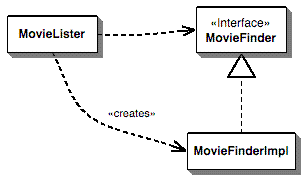
\includegraphics[width=2.1in]{1-Naive}
\caption{Vzniklé závislosti při naivní implementaci}
\label{fig:naive}
\end{figure}

Nyní je na čase využít Inversion of Control – pak již nebude třída MovieLister sama rozhodovat o tom, jakou implementaci použije, ale bude tuto informaci vyžadovat po okolí. Pomůže nám to také vyřešit problém s předáváním názvu souboru. V našem případě se zabýváme Dependency Injection, takže zvolíme tento typ IoC. Pro implementaci DI můžeme používat následující tři způsoby:

\begin{itemize}
\item{Constructor Injection} 
\item{Setter Injection} 
\item{Interface Injection} 
\end{itemize}

Všechny tři typy Dependency Injection mají společné to, že díky nim už nejsou „klientské“ třídy závislé na žádné konkrétní implementaci, ale pouze na obecném interface a čekají, že všechny potřebné parametry dostanou zvenku, dostáváme se tedy k situaci, kterou ilustruje \fig{injector}.

\begin{figure}[!ht]
\centering
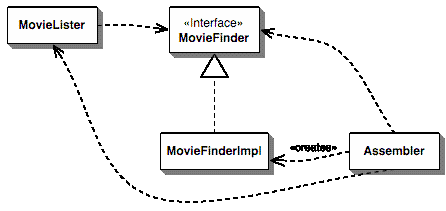
\includegraphics[width=3.2in]{2-Injector}
\caption{Závislosti při použití Dependency Injection}
\label{fig:injector}
\end{figure}

\subsection{Constructor Injection}

Při použití Constructor Injection definujeme závislosti třídy v konstruktoru, a tak vyžadujeme, aby bylo předáno vše, co třída potřebuje ke svému životu. Naše třídy tedy budou vypadat nějak takto:

\lstset{language=Java, caption=MovieLister s použitím Constructor Injection, label=listing:Java}
\begin{lstlisting}
class MovieLister...
    public MovieLister(MovieFinder finder) {
        this.finder = finder;       
    }

class ColonMovieFinder...
    public ColonDelimitedMovieFinder(String filename) {
        this.filename = filename;
    }
\end{lstlisting}

Nyní pokaždé, když budeme chtít instancovat třídu MovieLister, tak jí budeme muset dopředu předat konkrétní implementaci, kterou chceme zrovna použít. Jak je vidět, tak nyní jsme dosáhli oddělení místa použití a samotného skládání objektů, tento kód se tedy může objevit například v nějaké factory metodě:

\lstset{language=Java, caption=Příklad použití ve factory metodě, label=listing:Java}
\begin{lstlisting}
public MovieLister static createMovieLister() {
    MovieFinder finder = (MovieFinder) new ColonDelimitedMovieFinder("movies1.txt");
    MovieLister lister = new MovieLister(finder);
    return lister;
}
\end{lstlisting}

\subsection{Setter Injection}

Při použití Setter Injection nadefinujeme pro všechny závislosti, které potřebujeme dovnitř třídy předat, settery:

\lstset{language=Java, caption=MovieLister a Setter Injection, label=listing:Java}
\begin{lstlisting}
class MovieLister...
    private MovieFinder finder;
  public void setFinder(MovieFinder finder) {
    this.finder = finder;
  }

class ColonMovieFinder...
    private String filename;
    public void setFilename(String filename) {
        this.filename = filename;
    }
\end{lstlisting}

Kód, který nám připraví MovieLister tedy bude tentokrát vypadat takto:

\lstset{language=Java, caption=MovieLister Setter Injection a factory metoda, label=listing:Java}
\begin{lstlisting}
public MovieLister static createMovieLister() {
    ColonDelimitedMovieFinder finder = new ColonDelimitedMovieFinder();
    finder.setFilename("movies1.txt");
    MovieLister lister = new MovieLister();
    lister.setFinder(finder);
    return lister;
}
\end{lstlisting}

\subsection{Interface Injection}

U Interface Injection budeme podobně jako u Setter Injection definovat metody pro předání parametrů do našeho objektu, tentokrát ale jejich jméno určíme pomocí interface:

\lstset{language=Java,caption=Třída MovieLister implementující definované rozhraní,label=listing:Java}
\begin{lstlisting}
class MovieLister implements InjectFinder...
    private MovieFinder finder;
    public void injectFinder(MovieFinder finder) {
        this.finder = finder;
    }
\end{lstlisting}

Třída MovieLister pak musí toto rozhraní implementovat:

\lstset{language=Java,caption=Interface pro interface injection,label=listing:Java}
\begin{lstlisting}
public interface InjectFinder {
    void injectFinder(MovieFinder finder);
}
\end{lstlisting}

Identicky bude vypadat vložení filename do naší implementace MovieFinder.

\lstset{language=Java,caption=Implementace MovieLister u InterfaceInjection,label=listing:Java}
\begin{lstlisting}
public interface InjectFinderFilename {
    void injectFilename (String filename);
}
class ColonDelimitedMovieFinder implements MovieFinder, InjectFinderFilename......
    private String filename;
    public void injectFilename(String filename) {
        this.filename = filename;
    }
\end{lstlisting}

\section{Dependency Injection kontejner}
\label{sec:Container}

V ukázkách jednotlivých typů DI v první části byly objekty vždy sestavovány manuálně, tento kód je ale obdobný pro všechny případy, a tak tuto práci u DI můžeme přenechat tzv. kontejneru, kterému pouze poskytneme konfiguraci. Kontejner poté funguje vlastně tak, že sestaví a instancuje celý strom závislostí aplikace ještě předtím, než se samotná aplikace spustí. Můžeme si to představit na následujícím příkladu aplikace, mějme Controller, který bude používat nám již známou třídu MovieLister. Konstruktory jednotlivých tříd tedy budou vypadat nějak takto:

\lstset{language=Java,caption=Konstruktory tříd k příkladu,label=listing:Java}
\begin{lstlisting}
Controller (MovieLister lister) {...}
MovieLister(MovieFinder finder) {...}
MovieFinder(String filename) {...}
\end{lstlisting}

Pro to, abychom mohli spustit (tzn. nejdříve instancovat) náš Controller, tak již musíme předat všechny potřebné parametry – takže budeme vlastně postupovat opačně, zjišťovat závislosti a postupně sestavovat strom. Nejdříve tedy musíme instancovat MovieFinder, kterému předáme do parametru String. Movie Finder pak můžeme vložit do MovieListeru a ten teprve nakonec do Controlleru. Toto je samozřejmě velmi jednoduchý případ, pokud si ho ale představíme na složitější aplikaci, tak samozřejmě vzniklý strom bude daleko rozvětvenější.

\subsection{Dopady Dependency Injection na kód}

Dependency Injection by měl být pouze způsob, jak poskládat dohromady předem připravené třídy a tyto třídy by pokud možno uvnitř nemělo být potřeba měnit (někdy to zařídit ani nemůžeme – především u cizího kódu) a třídy by tak neměly o případném použití nějakého Dependency Injection kontejneru vůbec vědět. Když se podíváme na jednotlivé typy DI, tak největší nároky na podobu dané třídy klade Interface Injection, kde musíme vytvářet rozhraní a ta implementovat. U Setter Injection zase porušujeme čistý návrh objektu tím, že zveřejňujeme settery i pro parametry, které by měly zůstat po počáteční inicializaci neměnné – k tomu se nejlépe hodí Constructor Injection. Je zde velmi názorně patrné, které závislosti potřebuje třída pro svůj běh, a tak nemáme vlastně možnost třídu instancovat v nekonzistentní podobě. To zároveň nejlépe odpovídá požadavku na co nejmenší přizpůsobování se DI – třídu, která používá Constructor Injection bychom měli být schopní volně používat i bez jakéhokoli kontejneru a vždy mít zajištěnu její konzistentnost.
Naopak je zde několik problémů s využitím Constructor Injection:
\begin{itemize}
\item Pokud máme v konstruktoru hodně parametrů, tak může být méně přehledný, zvlášť výrazně je toto vidět u parametrů, které jsou skalárního typu (String, Integer), zde se pak můžeme orientovat pouze podle pořadí (u setterů vždy vidíme jméno toho, co nastavujeme).
\item Pokud máme více způsobů, jak sestavit daný objekt, tak můžeme poskytnout více konstruktorů, ty se ale můžou lišit pouze počtem a typy parametrů, takže nemusí vždy postačovat – pro ten případ pak můžeme použít factory metody nebo třídy.
\item Pokud máme více konstruktorů a ještě použijeme dědičnost, pak musíme vždy ošetřit všechny možnosti konstrukce a přesměrovat je na konstruktory rodiče, což může vést k ještě většímu počtu konstruktorů.
\end{itemize}
Navzdory zmíněným rizikům použití Constructor Injection bychom ji stále stejně jako Martin Fowler preferovali – její používání má nejmenší vliv na přirozené psaní tříd a také vždy zajišťuje konzistenci. Výběr není většinou tak zásadní, protože tvůrci jednotlivých kontejnerů a frameworků v mnoha případech podporují více typů DI, takže je možné v průběhu vývoje bez problémů přestoupit z Constructor Injection např. na Setter Injection, ostatně dalším dobrým důvodem pro podporu více typů DI je možnost integrace cizího kódu do naší aplikace, kde čím více typů je podporováno, tím je větší šance, že nenarazíme na situaci, kterou by daný kontejner nezvládl. Pro začlenění cizího kódu můžeme také využít návrhových vzorů jako např. Adapter nebo Bridge, které vhodně přizpůsobí rozhraní potřebě kontejneru.

\subsection{Services vs. Value Objects}

Pokud se podíváme na objekty, které tvoří naši aplikaci, můžeme zde nalézt dva základní druhy – objekty, které jsou zajímavé tím, že především vyjadřují svojí hodnotu (skalární typy jako string, integer, ale také doménové objekty) a dále pak objekty, které ty hodnotové pouze využívají a samotný vnitřní stav těchto objektů není tím důležitým. Máme tedy jednu sadu objektů, které reprezentují data a druhou skupinu, která slouží k manipulaci s těmito daty. K tomuto závěru došel Miško Hevery ve svém článku To „new“ or not to „new“ \cite{How to Think About the new Operator with Respect to Unit Testing}, hodnotové objekty označuje jako Newable (případně Value Object) a druhou skupinu jako Injectable (případně Service). Pojmy Injectable a Newable nejsou významově zcela přesné, jak si ukážeme na následujících řádcích, takže budou použity pojmy alternativní. Z tohoto rozdělení pak vyvozuje závěr, že Services by měly požadovat v konstruktoru (nebo jinou DI metodou) pouze další Services. Důvodem je to, že parametry Value Objects nejsou v momentě vytváření objektů DI kontejnerem ještě známy – kontejner nemůže vědět, jakou konkrétní hodnotu bude objekt mít v rámci naší aplikace. Podobně by Value Objects neměly ve svém konstruktoru vyžadovat objekty spadající do druhé skupiny. Services by obecně měly pracovat s Value Objects,takže opačná závislost by neměla být potřeba. Zároveň se nám tím velmi ulehčí mockování v Unit testech.
Pokud se podíváme na náš předchozí příklad, tak MovieLister jasně spadá do skupiny Services a ve svém konstruktoru si žádá pouze MovieFinder. Movie Finder spadá také do skupiny Services, ale v konstruktoru požaduje textový řetězec reprezentující název souboru. Jde sice o datový typ string, tzn. spadající do skupiny Value Object, ale tak, jak je příklad napsán, je tento parametr neměnný, a to znamená, že může být uveden přímo v konfiguračním souboru a je tedy přístupný už ve fázi, kdy kontejner skládá objekty dohromady.
Pro další ukázky budeme potřebovat více Value Objects, takže ve třídě MovieFinder budeme místo stringu požadovat objekt File:

\lstset{language=Java, caption=Value Object jako parametr v konstruktoru, label=listing:Java}
\begin{lstlisting}
class MovieFinder...
  public MovieFinder(File file) {
      ...
  }

class File...
  public File(String filename) {
      ...
  }
\end{lstlisting}

Pokud bychom nyní chtěli opět pro vybudování aplikace použít kontejner, tak bychom ho museli naučit, jak objekt File vybudovat. K tomu jsou určeny Factory třídy:

\lstset{language=Java, caption=Factory třída pro Value Object, label=listing:Java}
\begin{lstlisting}
class FileFactory...
  public File create(String filename) {
      return new File(filename);
  }
\end{lstlisting}

Pak už stačí pouze kontejner nakonfigurovat tak, aby objekt File vytvářel pomocí FileFactory a její metody create. Stejným způsobem pak doporučuji postupovat, pokud potřebujeme používat nějaký Value Object v nějaké Service – v konstruktoru požádáme o Factory třídu místo instance objektu a v momentě, kdy máme všechna potřebná data (například je teprve v této fázi dostaneme ze vstupu), teprve předáme parametry do Factory a dostaneme instanci. Výhodou tohoto způsobu oproti používání new na Value Objects (jak navrhuje Miško Hevery v odkazovaném článku\cite{How to Think About the new Operator with Respect to Unit Testing}) je možnost snadno měnit a konfigurovat implementaci nejen Services, ale i Value Objects. Factory třídy samozřejmě nemá cenu používat všude, je velmi nepravděpodobné, že bychom například potřebovali vyměnit implementaci rapper objektů jako String nebo Integer.

\subsection{Konfigurace}

Konfiguraci kontejneru – tzn. místo, kde určujeme, která konkrétní implementace se na daném místě použije, může mít v základu dvě podoby. První možností je tuto konfiguraci provést přímo pomocí programového kódu, nebo můžeme konfiguraci načítat z konfiguračního souboru a pak jej zpracovávat.
Výhodou konfiguračních souborů by mělo být to, že by je měl být schopný upravovat i někdo, kdo není programátor, což se ale asi moc často stávat nebude. Zásadnější však může být to, že nemusíme znovu kompilovat nějaký kód, pokud je potřeba pouze upravit konfiguraci.
Výhodnější může být zapsat konfiguraci pomocí kódu, pokud je konfigurace kratší – pak je zbytečné vytvářet konfigurační soubor. Nebo naopak pokud je konfigurace velmi komplexní a obsahuje nějakou podmiňovací logiku, pak není příliš vhodné takto „programovat“ v konfiguračním souboru.
Ve výsledku tato volba připadá na konkrétní situaci a preference programátorů. Ostatně pokud kontejner podporuje nastavení pomocí programového kódu, tak není výrazný problém si dopsat vlastní podporu pro nějaký typ konfiguračního souboru – například pokud bychom místo formátu XML chtěli použít YAML.

\subsection{Autowiring}

Autowiring se nazývá mechanismus, který by měl ulehčit konfiguraci DI kontejnerů. V různých implementacích nabízí různé možnosti, ale několik jich má společných – především ušetřit programátorovi psaní. Obecně Autowiring funguje tak, že se sám kontejner, případně jeho konfigurace snaží uhodnout určité parametry:
\begin{itemize}
\item U konstruktorů může Autowiring pomocí reflexe zjistit, které typy předáváme a pokud se tento typ vyskytuje v konstruktoru pouze jednou a zároveň má v systému jedinou implementaci, tak ji automaticky vybere.
\item Podobně se může chovat u properties dané třídy, kde může opět zjistit typ dané proměnné a podle něj uhodnout implementaci.
\item U properties se také někdy využívá odhadování podle jména proměnné, kdy pak systém hledá třídu, která má stejné jméno jako daná property.
\end{itemize}

Autowiring se tedy snaží použít informace, které jsme již uvedli při psaní kódu a pokud na jejich základě je schopný říci, jakou implementaci vložit, tak tuto informaci nemusíme duplikovat v konfiguraci. Samozřejmě nám ale nepomůže v případech, kdy potřebujeme do třídy injectovat např. parametry typu string – tam není, kde by danou hodnotu systém mohl zjistit a musíme ji zapsat sami.

\subsection{Konkrétní příklady}

\subsubsection{Spring}

Při použití Dependency Injection kontejneru, který je součástí Spring frameworku je potřeba všechny třídy, které chceme instancovat nadefinovat v XML souboru, přičemž závislosti mezi službami jsou nadefinovány jako „property“ element. Tyto informace Spring poté použije k zavolání správné „setter“ metody – jedná se totiž o kontejner, který používá Setter injection. Příklad konfiguračního souboru:

\lstset{language=XML,caption=Konfigurační soubor Spring kontejneru,label=listing:XML}
\begin{lstlisting}
<beans>  
	<bean id="AirlineAgency" class="com.dnene.ditutorial.common.impl.SimpleAirlineAgency" singleton="true"/>  
	<bean id="CabAgency" class="com.dnene.ditutorial.common.impl.SetterBasedCabAgency" singleton="true">  
		 <property name="airlineAgency">	
	 		<ref bean="AirlineAgency"/>   
		 </property>  
	 </bean> 
	 <bean id="TripPlanner" class="com.dnene.ditutorial.common.impl.SetterBasedTripPlanner" singleton="true">   
	 	<property name="airlineAgency">	
			<ref bean="AirlineAgency"/>   
		</property>   
		<property name="cabAgency">	
			<ref bean="CabAgency"/>   
		</property>  
	</bean> 
</beans>
\end{lstlisting}

Při inicializaci kontejneru je potřeba poskytnout název konfiguračního souboru:

\lstset{language=Java,caption=Inicializace kontejneru,label=listing:Java}
\begin{lstlisting}
ClassPathResource res = new ClassPathResource("spring-beans.xml"); BeanFactory factory = new XmlBeanFactory(res);
\end{lstlisting}

Jednotlivé služby pak v kódu získáváme prostřednictvím id atributů definovaných v XML konfiguračním souboru. Stejně jako u jiných kontejnerů, i zde jsou třídy nainstancovány ve správném pořadí a závislosti jsou do nich vloženy prostřednictvím nadefinovaných setterů.

\lstset{language=Java,caption=Inicializace kontejneru,label=listing:Java}
\begin{lstlisting}
factory.getBean("TripPlanner");
\end{lstlisting}

\subsubsection{PicoContainer}

Pro použití PicoContaineru je potřeba nejprve instancovat  DefaultPicoContainer

\lstset{language=Java,caption=Inicializace kontejneru,label=listing:Java}
\begin{lstlisting}
pico = new DefaultPicoContainer();
\end{lstlisting}

Následně je potřeba zaregistrovat jednotlivé třídy:

\lstset{language=Java,caption=Registrace tříd v kontejneru,label=listing:Java}
\begin{lstlisting}
pico.registerComponentImplementation(SimpleAirlineAgency.class); pico.registerComponentImplementation(ConstructorBasedCabAgency.class); pico.registerComponentImplementation(ConstructorBasedTripPlanner.class);
\end{lstlisting}

PicoContainer je příkladem Constructor injection (podporuje i setter injection, ale constructor injection je u tohoto kontejneru preferovaná) a v kódu vypadá například takto:

\lstset{language=Java,caption=Použití PicoContainer,label=listing:Java}
\begin{lstlisting}
public ConstructorBasedCabAgency(AirlineAgency airlineAgency) {  this.airlineAgency = airlineAgency; }
\end{lstlisting}

Třída ConstructorBasedCabAgency je tedy závislá na rozhraní AirlineAgency a zároveň ConstructorBasedTripPlanner je závislý na CabAgency a také AirlineAgency.
PicoContainer rozhoduje závislosti prohlížením jednotlivých konstruktorů, přičemž jednotlivé služby se u něj registrují prostřednictvím implementovaných tříd, klient si ovšem o službu říká prostřednictvím názvu rozhraní. PicoContainer následně traverzuje celou implementační hierarchií rozhraní a vybere nejvhodnější třídu.
U předešlého příkladu je tedy TripPlanner závislý na AirlineAgency a CabAgency a AirlineAgency a CabAgency jsou závislé na TripPlanner. PicoContainer tedy nejprve nainstancuje AirlineAgency, předá referenci konstruktoru CabAgency a poté předá CabAgency i AirlineAgency při vytváření TripPlanneru. Celou tuto sekvenci vyvoláme následujícím příkazem: pico.getComponentInstanceOfType(TripPlanner.class).

\section{Service locator}

Alternativní implementací IoC je vzor ServiceLocator (SL), stejně jako DI slouží ke snížení závislostí mezi požadovanou funkčností a konkrétní implementací. Service Locator pracuje tak, že uvnitř sebe (podobný kontejner jako u DI) nese informaci o tom, jaké rozhraní je implementováno jakou třídou. Pokaždé když v nějaké třídě potřebujeme přistoupit k jiné, tak požádáme SL, aby nám vyrobil příslušný objekt. V našem příkladě tedy u třídy MovieLister zmizí závislost na konkrétní implementaci MovieFinder, zůstane závislost na rozhraní MovieFinder a ještě k tomu přibyde závislost na rozhraní Service Locatoru, viz \fig{locator}.

\begin{figure}[!ht]
\centering
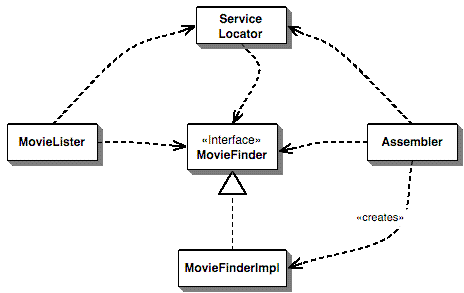
\includegraphics[width=3.5in]{3-Locator}
\caption{Zobrazení závislostí při použití Service Locatoru}
\label{fig:locator}
\end{figure}

Následuje ukázka, jak by mohl vypadat MovieLister v případě, že je Service Locator implementován jako Singleton. Ten má na sobě definované metody pro přídem a výdej objektů, což nemusí být ideální, ale zde to pro ilustraci postačuje.

\lstset{language=Java, caption=MovieLister při použití Service Locatoru, label=listing:Java}
\begin{lstlisting}
class MovieLister ... { 
  private MovieFinder finder;
  public MovieLister() {
    this.finder = ServiceLocator.getMovieFinder();
  }
\end{lstlisting}

Rozdílem mezi oběma představenými implementacemi IoC je to, že v případě DI třída pouze deklaruje, která rozhraní potřebuje a to, jakým způsobem a kdy je dostane, tak nijak neovlivňuje. Naopak u tříd využívajících SL vždy voláme kontejner na konkrétním místě. Velkou nevýhodou je také, že každá třída, která SL využívá, tak je závislá na jeho rozhraní (případně můžeme definovat částečná rozhraní pro jednotlivé služby, které SL vydává, ale závislost stejně zůstává). Pokud máme vytvořit nějaké hodně obecné třídy, tak v nich tato závislost zůstane, tak by pro využití s jiným SL kontejnerem musel využít nějaký adaptér. Z hlediska dopadu na kód, které bylo diskutováno v předchozích částech, tak je SL jednoznačně invazivnější než DI. S tím souvisí i čitelnost kódu - u Dependency Injection, zvláště pokud použijeme nejčistší Constructor Injection metodu, tak vidíme zcela přesně všechny závislosti, které třída má na první pohled. U Service Locatoru bychom pro dosažení stejného cíle museli prohlédnout celý kód třídy, protože volání Service Locatoru se může vyskytnout kdekoli v kódu.

% conference papers do not normally have an appendix


% use section* for acknowledgement
% \section*{Acknowledgment}
% 
% 
% We would like to thank Michael Jeff Donahoo for his valuable advice and comments.
% We would also like to thank Bozena Mannova for her early feedback that motivated
% our work.
% 
% 




% trigger a \newpage just before the given reference
% number - used to balance the columns on the last page
% adjust value as needed - may need to be readjusted if
% the document is modified later
%\IEEEtriggeratref{8}
% The "triggered" command can be changed if desired:
%\IEEEtriggercmd{\enlargethispage{-5in}}

% references section

% can use a bibliography generated by BibTeX as a .bbl file
% BibTeX documentation can be easily obtained at:
% http://www.ctan.org/tex-archive/biblio/bibtex/contrib/doc/
% The IEEEtran BibTeX style support page is at:
% http://www.michaelshell.org/tex/ieeetran/bibtex/
%\bibliographystyle{IEEEtran}
% argument is your BibTeX string definitions and bibliography database(s)
%\bibliography{IEEEabrv,../bib/paper}
%
% <OR> manually copy in the resultant .bbl file
% set second argument of \begin to the number of references
% (used to reserve space for the reference number labels box)
\begin{thebibliography}{1}

\bibitem{Inversion of Control Containers and the Dependency Injection pattern}
Martin Fowler, http://martinfowler.com/articles/injection.html
\bibitem{Spring - The IoC container}
Spring, http://static.springsource.org/spring/docs/2.5.x/reference/beans.html
\bibitem{How to Think About the new Operator with Respect to Unit Testing}
Misko Hevery, http://misko.hevery.com/2008/07/08/how-to-think-about-the-new-operator/
\bibitem{To new or not to new...}
Misko Hevery, http://misko.hevery.com/2008/09/30/to-new-or-not-to-new/
\bibitem{Dependency Injection Zendcon 2010}
Fabien Potencier, http://www.slideshare.net/fabpot/dependency-injectionzendcon2010
\bibitem{A beginners guide to Dependency Injection}
Dhananjay Nene, http://www.theserverside.com/news/1321158/A-beginners-guide-to-Dependency-Injection

\end{thebibliography}




% that's all folks
\end{document}



